%package list
\documentclass{article}
\usepackage[top=3cm, bottom=3cm, outer=3cm, inner=3cm]{geometry}
\usepackage{multicol}
\usepackage{graphicx}
\usepackage{url}
%\usepackage{cite}
\usepackage{hyperref}
\usepackage{array}
%\usepackage{multicol}
\newcolumntype{x}[1]{>{\centering\arraybackslash\hspace{0pt}}p{#1}}
\usepackage{natbib}
\usepackage{pdfpages}
\usepackage{multirow}
\usepackage[normalem]{ulem}
\useunder{\uline}{\ul}{}
\usepackage{svg}
\usepackage{xcolor}
\usepackage{listings}
\usepackage{enumitem}
\usepackage{amsmath}
\lstdefinestyle{ascii-tree}{
    literate={├}{|}1 {─}{--}1 {└}{+}1 
  }
\lstset{basicstyle=\ttfamily,
  showstringspaces=false,
  commentstyle=\color{red},
  keywordstyle=\color{blue}
}
%\usepackage{booktabs}
\usepackage{caption}
\usepackage{subcaption}
\usepackage{float}
\usepackage{array}

\newcolumntype{M}[1]{>{\centering\arraybackslash}m{#1}}
\newcolumntype{N}{@{}m{0pt}@{}}


%%%%%%%%%%%%%%%%%%%%%%%%%%%%%%%%%%%%%%%%%%%%%%%%%%%%%%%%%%%%%%%%%%%%%%%%%%%%
%%%%%%%%%%%%%%%%%%%%%%%%%%%%%%%%%%%%%%%%%%%%%%%%%%%%%%%%%%%%%%%%%%%%%%%%%%%%
\newcommand{\itemStudent}{%
    \begin{minipage}[t]{0.9\linewidth}
        - David Alfredo Huamani Ollachica \\
        - Marco Antonio Suarez Huamaní \\
        - Rafael Diego Nina Calizaya \\
        - Angel Paul Apaza Nazareth
    \end{minipage}%
}

\newcommand{\itemCourse}{Programación Web 2}
\newcommand{\itemCourseCode}{1702122}
\newcommand{\itemSemester}{III}
\newcommand{\itemUniversity}{Universidad Nacional de San Agustín de Arequipa}
\newcommand{\itemFaculty}{Facultad de Ingeniería de Producción y Servicios}
\newcommand{\itemDepartment}{Departamento Académico de Ingeniería de Sistemas e Informática}
\newcommand{\itemSchool}{Escuela Profesional de Ingeniería de Sistemas }
\newcommand{\itemAcademic}{2024 - A}
\newcommand{\itemInput}{Del 3 Junio 2024}
\newcommand{\itemOutput}{Al 7 Junio 2024}
\newcommand{\itemPracticeNumber}{06}
\newcommand{\itemTheme}{Django (Admin)}
%%%%%%%%%%%%%%%%%%%%%%%%%%%%%%%%%%%%%%%%%%%%%%%%%%%%%%%%%%%%%%%%%%%%%%%%%%%%
%%%%%%%%%%%%%%%%%%%%%%%%%%%%%%%%%%%%%%%%%%%%%%%%%%%%%%%%%%%%%%%%%%%%%%%%%%%%

\usepackage[english,spanish]{babel}
\usepackage[utf8]{inputenc}
\AtBeginDocument{\selectlanguage{spanish}}
\renewcommand{\figurename}{Figura}
\renewcommand{\refname}{Referencias}
\renewcommand{\tablename}{Tabla} %esto no funciona cuando se usa babel
\AtBeginDocument{%
	\renewcommand\tablename{Tabla}
}

\usepackage{fancyhdr}
\pagestyle{fancy}
\fancyhf{}
\setlength{\headheight}{30pt}
\renewcommand{\headrulewidth}{1pt}
\renewcommand{\footrulewidth}{1pt}
\fancyhead[L]{\raisebox{-0.2\height}{
\includegraphics[width=3cm]{img/logo_episunsa.png}}}
\fancyhead[C]{\fontsize{7}{7}\selectfont	\itemUniversity \\ \itemFaculty \\ \itemDepartment \\ \itemSchool \\ \textbf{\itemCourse}}
\fancyhead[R]{\raisebox{-0.2\height}{
\includegraphics[width=1.2cm]{img/logo_abet}}}
\fancyfoot[L]{Grupo 3 - PW2}
\fancyfoot[C]{\itemCourse}
\fancyfoot[R]{Página \thepage}

% para el codigo fuente
\usepackage{listings}
\usepackage{color, colortbl}
\definecolor{dkgreen}{rgb}{0,0.6,0}
\definecolor{gray}{rgb}{0.5,0.5,0.5}
\definecolor{mauve}{rgb}{0.58,0,0.82}
\definecolor{codebackground}{rgb}{0.95, 0.95, 0.92}
\definecolor{tablebackground}{rgb}{0.8, 0, 0}

\lstset{frame=tb,
	language=Python,
	aboveskip=3mm,
	belowskip=3mm,
	showstringspaces=false,
	columns=flexible,
	basicstyle={\small\ttfamily},
	numbers=none,
	numberstyle=\tiny\color{gray},
	keywordstyle=\color{blue},
	commentstyle=\color{dkgreen},
	stringstyle=\color{mauve},
	breaklines=true,
	breakatwhitespace=true,
	tabsize=4,
	backgroundcolor= \color{codebackground},
}

\begin{document}
	
	\vspace*{10px}
	
	\begin{center}	
		\fontsize{17}{17} \textbf{ Informe de Laboratorio \itemPracticeNumber}
	\end{center}
	\centerline{\textbf{\Large Tema: \itemTheme}}
	%\vspace*{0.5cm}	

	\begin{flushright}
		\begin{tabular}{|M{2.5cm}|N|}
			\hline 
			\rowcolor{tablebackground}
			\color{white} \textbf{Nota}  \\
			\hline 
			     \\[30pt]
			\hline 			
		\end{tabular}
	\end{flushright}	

	\begin{table}[H]
		\begin{tabular}{|x{4.7cm}|x{4.8cm}|x{4.8cm}|}
			\hline 
			\rowcolor{tablebackground}
			\color{white} \textbf{Estudiante} & \color{white}\textbf{Escuela}  & \color{white}\textbf{Asignatura}   \\
			\hline 
			{\itemStudent } & \itemSchool & {\itemCourse \par Semestre: \itemSemester \par Código: \itemCourseCode}     \\ 
			\hline 			
		\end{tabular}
	\end{table}		
	
	\begin{table}[H]
		\begin{tabular}{|x{4.7cm}|x{4.8cm}|x{4.8cm}|}
			\hline 
			\rowcolor{tablebackground}
			\color{white}\textbf{Laboratorio} & \color{white}\textbf{Tema}  & \color{white}\textbf{Duración}   \\
			\hline 
			\itemPracticeNumber & \itemTheme & 04 horas   \\
			\hline 
		\end{tabular}
	\end{table}
	
	\begin{table}[H]
		\begin{tabular}{|x{4.7cm}|x{4.8cm}|x{4.8cm}|}
			\hline 
			\rowcolor{tablebackground}
			\color{white}\textbf{Semestre académico} & \color{white}\textbf{Fecha de inicio}  & \color{white}\textbf{Fecha de entrega}   \\
			\hline 
			\itemAcademic & \itemInput &  \itemOutput  \\
			\hline 
		\end{tabular}
	\end{table}
	
	\section{Tarea}
	
\begin{itemize}
    \item URL GitHub del Projecto Django \url{https://github.com/DrN25/Grupo3_Project}
		  \begin{lstlisting}[language=bash,caption={imagen de los commits realizados}][H]
git log --graph --pretty=oneline --abbrev-commit --all
* 3c41634 (HEAD -> main, origin/main, origin/HEAD) Creando el modelo ProductoPedido
* 70a9a92 Creando el modelo Pedido
* ca40354 Creando el modelo CarritoCompras
* 804c902 Creando el modelo Publicacion
* 4d8c94b Creando el modelo Comentario
* 52ad431 Creando el modelo Producto
* 3d59528 Creando el modelo Categoria
* 099166b Creando el modelo Vendedor
* 1d111fb Creando el modelo Usuario
* 57983d0 Primer commit
		  \end{lstlisting}
    
\end{itemize}


	\section{Modelo de la base de datos}
	
	\subsection{Idea de proyecto}
	\begin{itemize}	
                \item Nuestro proyecto consiste en desarrollar una tienda virtual que permita a los usuarios explorar y adquirir productos de manera sencilla y eficiente. La plataforma ofrecerá una experiencia de compra intuitiva, con características como búsqueda avanzada de productos, carrito de compras, procesamiento seguro de pagos y gestión de cuentas de usuarios. Además, proporcionará a los administradores herramientas para gestionar inventarios, pedidos y promociones, por ultimo incluye un sistema tipo red social para que los demas compradores vean y reaccionen a comentarios en las publicaciones que hacen los vendedores sobre sus productos, asegurando un manejo óptimo del negocio y una experiencia de usuario satisfactoria.

                \item Inspiraciones: \href{https://www.mercadolibre.com}{MercadoLibre} y \href{https://www.amazon.com}{Amazon}
\begin{figure}[h]
    \centering
    \begin{subfigure}[b]{0.45\linewidth}
        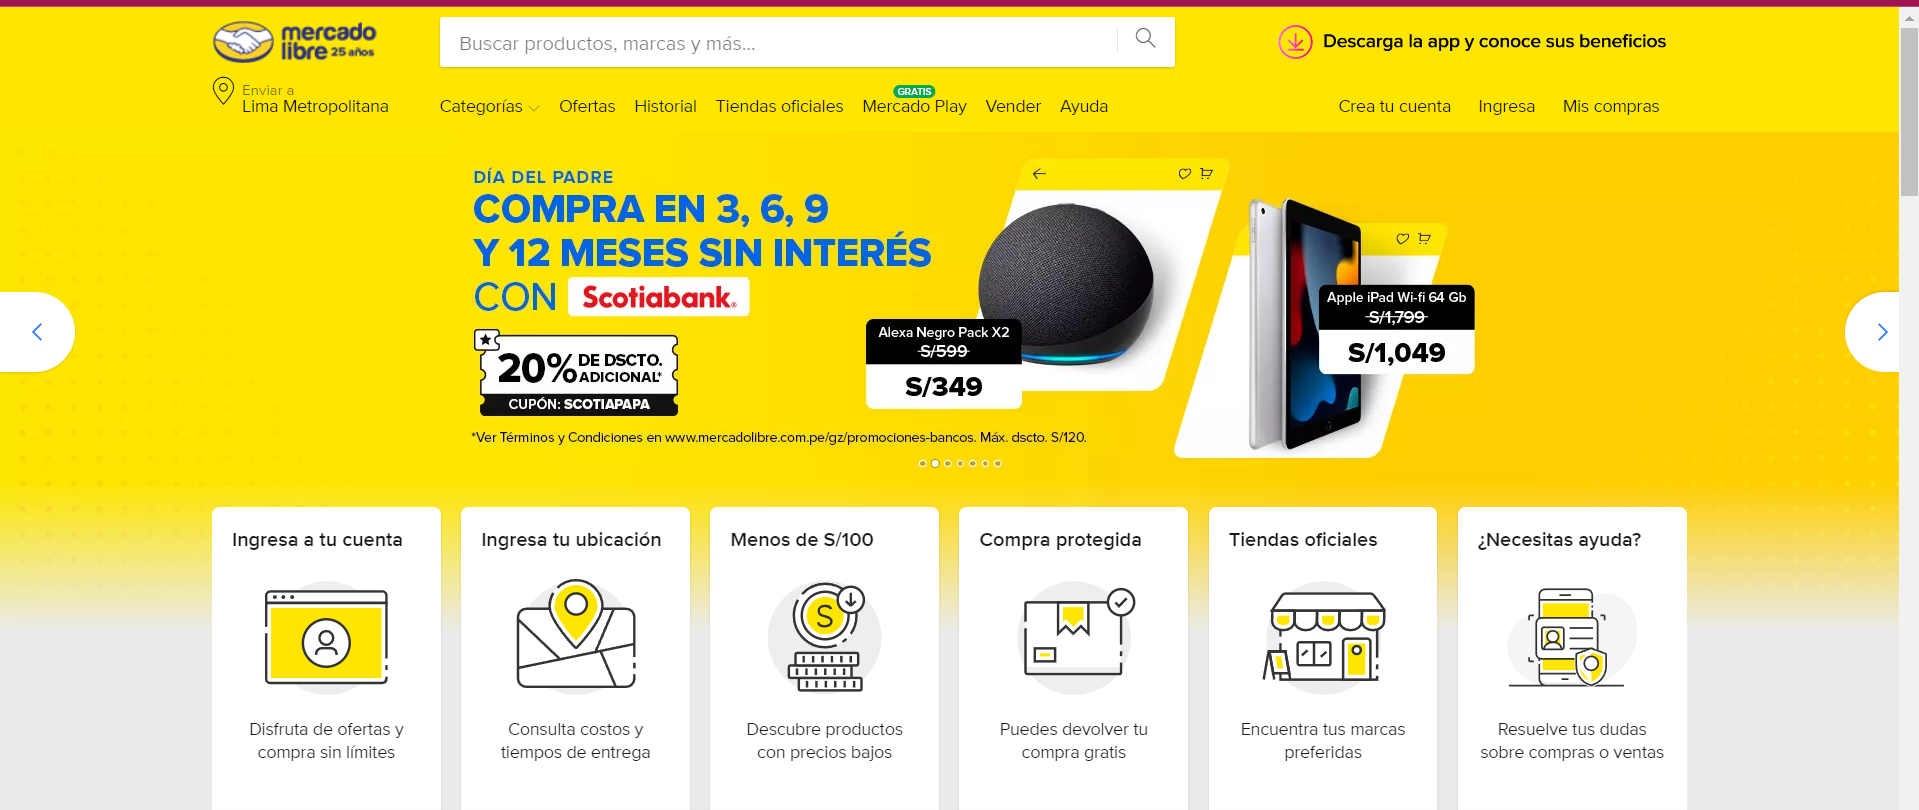
\includegraphics[width=\linewidth]{img/ins1.png}
        \caption{Mercado Libre}
        \label{fig:ejercicioA}
    \end{subfigure}
    \hfill
    \begin{subfigure}[b]{0.45\linewidth}
        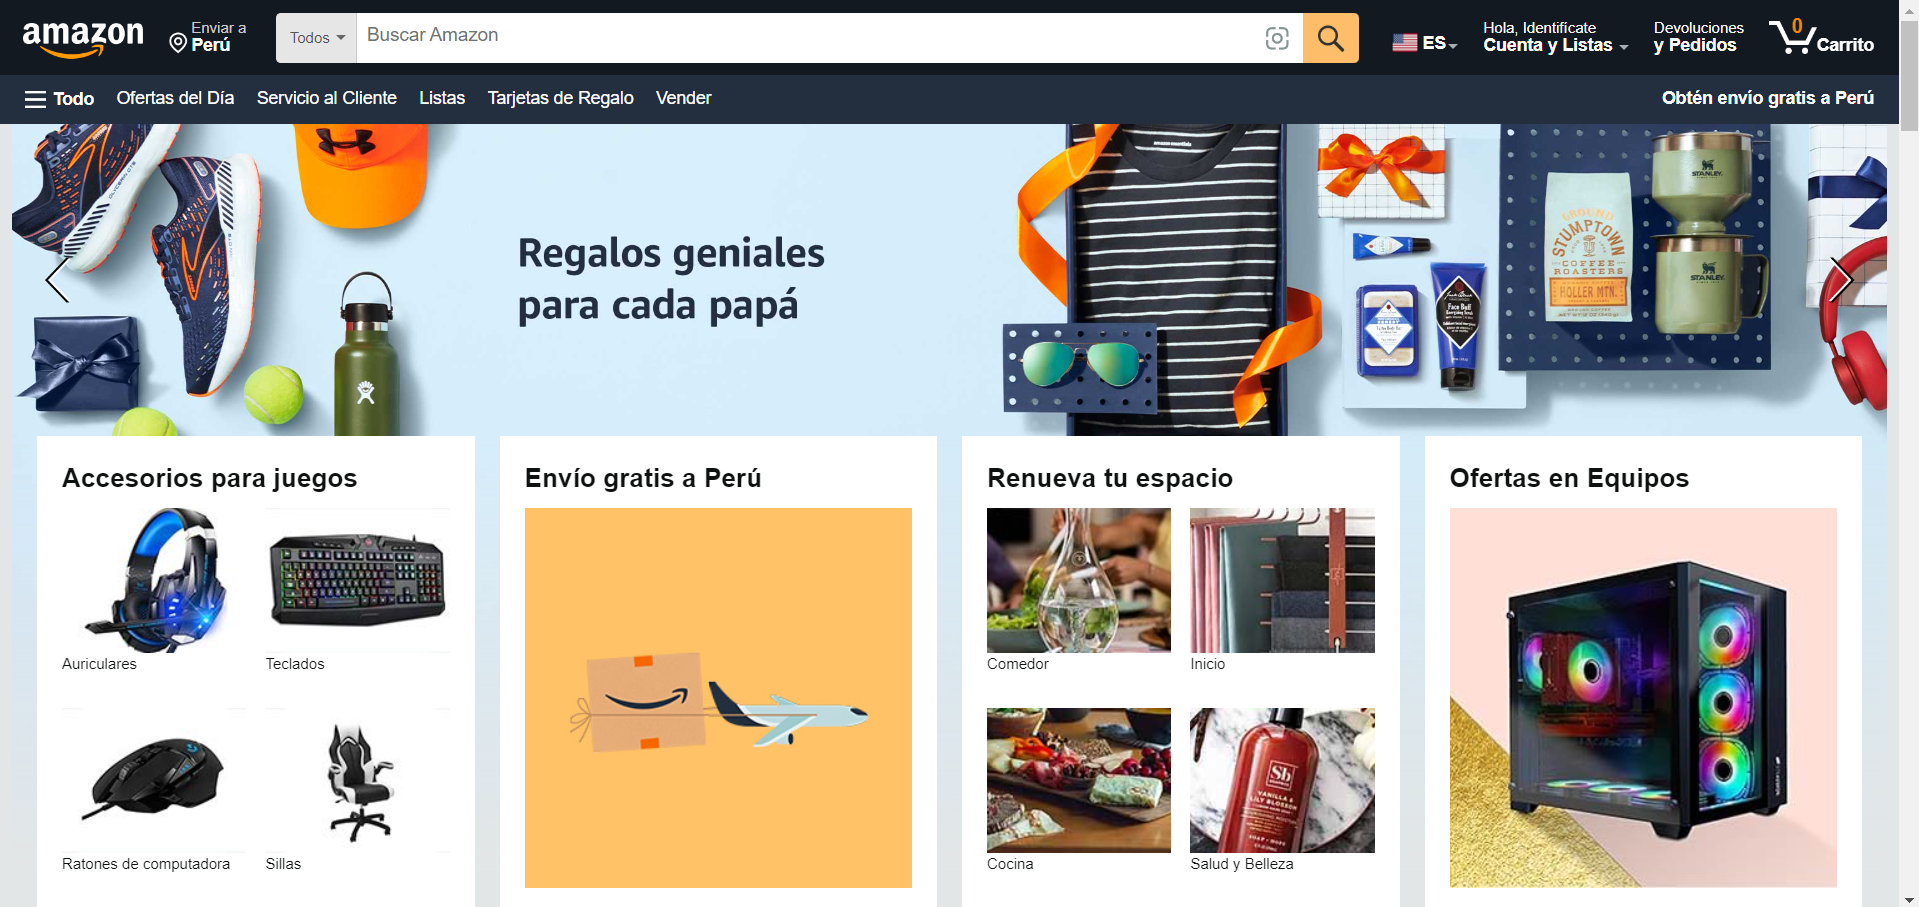
\includegraphics[width=\linewidth]{img/ins2.png}
        \caption{Amazon}
        \label{fig:ejercicioB}
    \end{subfigure}
    \caption{Implementación y ejecución de los ejercicios}
    \label{fig:ejercicios}
\end{figure}
	\end{itemize}	

  
	\subsection{Modelo de base de datos}
	\begin{itemize}	
            \item Para el modelo de la base de datos se incluyeron las siguientes tablas:
            
            \section*{Esquema de la Base de Datos}

\subsection*{Tabla \texttt{Pedido}}
\begin{itemize}[leftmargin=*]
    \item \textbf{idPedido}: Identificador único del pedido.
    \item \textbf{payMethod}: Método de pago utilizado para el pedido.
    \item \textbf{total}: Total del pedido.
    \item \textbf{date}: Fecha del pedido.
    \item \textbf{idUsuario}: Clave foránea que referencia al usuario que realizó el pedido.
    \item \textbf{idVendedor}: Clave foránea que referencia al vendedor asociado al pedido.
    \item \textbf{idProductoPedido}: Clave foránea que referencia al producto asociado al pedido.
\end{itemize}

\subsection*{Tabla \texttt{ProductoPedido}}
\begin{itemize}[leftmargin=*]
    \item \textbf{idProductoPedido}: Identificador único del producto en el pedido.
    \item \textbf{amount}: Cantidad del producto en el pedido.
    \item \textbf{total}: Total del producto en el pedido.
    \item \textbf{idProducto}: Clave foránea que referencia al producto asociado al pedido.
\end{itemize}

\subsection*{Tabla \texttt{Usuario}}
\begin{itemize}[leftmargin=*]
    \item \textbf{idUsuario}: Identificador único del usuario.
    \item \textbf{name}: Nombre del usuario.
    \item \textbf{email}: Correo electrónico del usuario.
    \item \textbf{phone}: Número de teléfono del usuario.
    \item \textbf{password}: Contraseña del usuario.
    \item \textbf{address}: Dirección del usuario.
\end{itemize}

\subsection*{Tabla \texttt{CarritoCompras}}
\begin{itemize}[leftmargin=*]
    \item \textbf{idCarrito}: Identificador único del carrito de compras.
    \item \textbf{total}: Total del carrito de compras.
    \item \textbf{status}: Estado del carrito de compras.
    \item \textbf{idUsuario}: Clave foránea que referencia al usuario asociado al carrito de compras.
    \item \textbf{idProducto}: Clave foránea que referencia al producto asociado al carrito de compras.
\end{itemize}

\subsection*{Tabla \texttt{Producto}}
\begin{itemize}[leftmargin=*]
    \item \textbf{idProducto}: Identificador único del producto.
    \item \textbf{name}: Nombre del producto.
    \item \textbf{weight}: Peso del producto.
    \item \textbf{unitPrice}: Precio unitario del producto.
    \item \textbf{stocj}: Stock del producto.
    \item \textbf{idCategoria}: Clave foránea que referencia a la categoría del producto.
    \item \textbf{idVendedor}: Clave foránea que referencia al vendedor asociado al producto.
\end{itemize}

\subsection*{Tabla \texttt{Categoria}}
\begin{itemize}[leftmargin=*]
    \item \textbf{idCategoria}: Identificador único de la categoría.
    \item \textbf{name}: Nombre de la categoría.
\end{itemize}

\subsection*{Tabla \texttt{Vendedor}}
\begin{itemize}[leftmargin=*]
    \item \textbf{idVendedor}: Identificador único del vendedor.
    \item \textbf{name}: Nombre del vendedor.
    \item \textbf{email}: Correo electrónico del vendedor.
    \item \textbf{phone}: Número de teléfono del vendedor.
    \item \textbf{password}: Contraseña del vendedor.
    \item \textbf{address}: Dirección del vendedor.
    \item \textbf{description}: Descripción del vendedor.
    \item \textbf{perfilPhoto}: Foto de perfil del vendedor.
\end{itemize}

\subsection*{Tabla \texttt{Publicacion}}
\begin{itemize}[leftmargin=*]
    \item \textbf{idPublicacion}: Identificador único de la publicación.
    \item \textbf{likes}: Número de likes de la publicación.
    \item \textbf{dislikes}: Número de dislikes de la publicación.
    \item \textbf{idVendedor}: Clave foránea que referencia al vendedor asociado a la publicación.
    \item \textbf{idProducto}: Clave foránea que referencia al producto asociado a la publicación.
    \item \textbf{idComentario}: Clave foránea que referencia al comentario asociado a la publicación.
\end{itemize}

\subsection*{Tabla \texttt{Comentario}}
\begin{itemize}[leftmargin=*]
    \item \textbf{idComentario}: Identificador único del comentario.
    \item \textbf{content}: Contenido del comentario.
    \item \textbf{date}: Fecha del comentario.
    \item \textbf{idUsuario}: Clave foránea que referencia al usuario que realizó el comentario.
\end{itemize}

    \subsection*{Diagrama E-R}
    


            \begin{figure}[h]
                \centering
                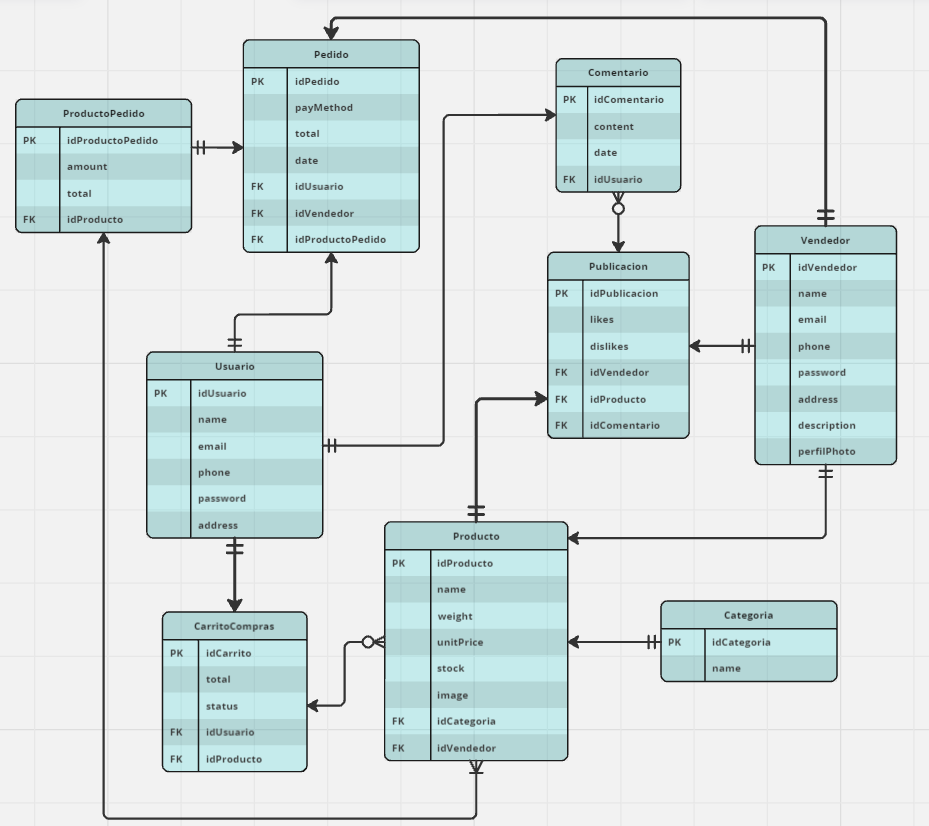
\includegraphics[width=0.8\textwidth]{img/model.png}
                \caption{Modelo de la Base de Datos}
                \label{fig:modelo_bd}
            \end{figure}
            

	\end{itemize}	
\vspace{10cm}

  	\subsection{Codigo en el projecto Django Python}
\begin{itemize}
    \item A continuacion se muestran los modelos ya implementados en python.
\end{itemize}
\subsection*{Modelo \texttt{Carrito de compras}}
		  \begin{lstlisting}[language=Python,caption={CarritoCompras.py}][H]
  from django.db import models
from django.utils.translation import gettext_lazy as _
import uuid

from .Usuario import Usuario
from .Producto import Producto

class CarritoCompras(models.Model):
    idCarrito = models.UUIDField(primary_key=True, default=uuid.uuid4, editable=False)
    total = models.DecimalField(null=False, blank=False, max_digits=10, decimal_places=2, default=0)
    STATUS = [
        ('empty','empty'),
        ('in_process','in process'),
        ('completed','completed')
    ]
    status = models.CharField(null=False, max_length=10, choices=STATUS, default='empty')
    idUsuario = models.ForeignKey(Usuario, on_delete=models.CASCADE)
    idProducto = models.ForeignKey(Producto, on_delete=models.CASCADE, blank=True, null=True)

    class Meta:
        ordering = ['status', 'idUsuario', 'idProducto']

    def save(self, *args, **kwargs):
        self.status = self.status.upper()
        return super(CarritoCompras, self).save(*args, **kwargs)

    def __str__(self):
        return "%s %s %s" % (self.status, self.idUsuario, self.idProducto)
    \end{lstlisting}

\subsection*{Modelo \texttt{Categoria}}
		  \begin{lstlisting}[language=Python,caption={Categoria.py}][H]
from django.db import models
from django.utils.translation import gettext_lazy as _
import uuid

class Categoria(models.Model):
    idCategoria = models.UUIDField(primary_key=True, default=uuid.uuid4, editable=False)
    name = models.CharField(null=False, blank=False, max_length=255)

    class Meta:
        ordering = ['name']

    def save(self, *args, **kwargs):
        self.name = self.name.upper()
        return super(Categoria, self).save(*args, **kwargs)

    def __str__(self):
        return "%s" % (self.name)
    \end{lstlisting}

\subsection*{Modelo \texttt{Comentario}}
		  \begin{lstlisting}[language=Python,caption={Comentario.py}][H]
from django.db import models
from django.utils.translation import gettext_lazy as _
import uuid

from .Usuario import Usuario

class Comentario(models.Model):
    idComentario = models.UUIDField(primary_key=True, default=uuid.uuid4, editable=False)
    content = models.CharField(null=False, blank=False, max_length=255)
    date = models.DateTimeField(editable=False, null=False, auto_now_add=True)
    idUsuario = models.ForeignKey(Usuario, on_delete=models.CASCADE)

    class Meta:
        ordering = ['idUsuario', 'content']

    def save(self, *args, **kwargs):
        self.content = self.content.upper()
        return super(Comentario, self).save(*args, **kwargs)

    def __str__(self):
        return "%s %s" % (self.idUsuario, self.date)
    \end{lstlisting}


\subsection*{Modelo \texttt{Pedido}}
		  \begin{lstlisting}[language=Python,caption={Pedido.py}][H]
from django.db import models
from django.utils.translation import gettext_lazy as _
import uuid

from .Usuario import Usuario
from .Vendedor import Vendedor
from .ProductoPedido import ProductoPedido

class Pedido(models.Model):
    idPedido = models.UUIDField(primary_key=True, default=uuid.uuid4, editable=False)
    METODO_PAGO = [
        ('credito','Tarjeta de Credito'),
        ('debito','Tarjeta de Debito'),
        ('paypal','Paypal'),
        ('otro','Otros')
    ]
    payMethod = models.CharField(null=False, max_length=20, choices=METODO_PAGO, default='credito')
    total = models.DecimalField(null=False, blank=False, max_digits=10, decimal_places=2, default=0.00)
    date = models.DateTimeField(editable=False, null=False, auto_now_add=True)
    idUsuario = models.ForeignKey(Usuario, on_delete=models.CASCADE)
    idVendedor = models.ForeignKey(Vendedor, on_delete=models.CASCADE)
    idProductoPedido = models.ForeignKey(ProductoPedido, on_delete=models.CASCADE)

    class Meta:
        ordering = ['idUsuario', 'idVendedor', 'idProductoPedido', 'total', 'date']

    def save(self, *args, **kwargs):
        self.payMethod = self.payMethod.upper()
        return super(Pedido, self).save(*args, **kwargs)

    def __str__(self):
        return "%s %s" % (self.idUsuario, self.total)
    \end{lstlisting}


\subsection*{Modelo \texttt{Producto}}
		  \begin{lstlisting}[language=Python,caption={Producto.py}][H]
from django.db import models
from django.utils.translation import gettext_lazy as _
import uuid

from .Categoria import Categoria
from .Vendedor import Vendedor

class Producto(models.Model):
    idProducto = models.UUIDField(primary_key=True, default=uuid.uuid4, editable=False)
    name = models.CharField(null=False, blank=False, max_length=255)
    weight = models.DecimalField(null=True, blank=True, max_digits=10, decimal_places=2)
    unitPrice = models.DecimalField(null=False, blank=False, max_digits=10, decimal_places=2)
    stock = models.IntegerField(null=False, blank=False)
    image = models.ImageField(upload_to='image_photos/', null=True, blank=True)
    idCategoria = models.ForeignKey(Categoria, on_delete=models.CASCADE)
    idVendedor = models.ForeignKey(Vendedor, on_delete=models.CASCADE)

    class Meta:
        ordering = ['name', 'unitPrice', 'stock', 'idCategoria', 'idVendedor']

    def save(self, *args, **kwargs):
        self.name = self.name.upper()
        return super(Producto, self).save(*args, **kwargs)

    def __str__(self):
        return "%s %s %s %s %s" % (self.name, self.unitPrice, self.stock, self.idCategoria, self.idVendedor)
    \end{lstlisting}

\subsection*{Modelo \texttt{Producto Pedido}}
		  \begin{lstlisting}[language=Python,caption={ProductoPedido.py}][H]
from django.db import models
from django.utils.translation import gettext_lazy as _
import uuid

from .Producto import Producto

class ProductoPedido(models.Model):
    idPedido = models.UUIDField(primary_key=True, default=uuid.uuid4, editable=False)
    amount = models.IntegerField(null=False, blank=False)
    total = models.DecimalField(null=False, blank=False, max_digits=10, decimal_places=2, default=0.00)
    idProducto = models.ForeignKey(Producto, on_delete=models.CASCADE)

    class Meta:
        ordering = ['idProducto', 'amount', 'total']

    def save(self, *args, **kwargs):
        return super(ProductoPedido, self).save(*args, **kwargs)

    def __str__(self):
        return "%s %s %s" % (self.idProducto, self.amount, self.total)
    \end{lstlisting}

\subsection*{Modelo \texttt{Publicacion}}
		  \begin{lstlisting}[language=Python,caption={Publicacion.py}][H]
from django.db import models
from django.utils.translation import gettext_lazy as _
import uuid

from .Producto import Producto
from .Vendedor import Vendedor
from .Comentario import Comentario

class Publicacion(models.Model):
    idPublicacion = models.UUIDField(primary_key=True, default=uuid.uuid4, editable=False)
    likes = models.IntegerField(null=False, blank=False, default=0)
    dislikes = models.IntegerField(null=False, blank=False, default=0)
    idVendedor = models.ForeignKey(Vendedor, on_delete=models.CASCADE)
    idProducto = models.ForeignKey(Producto, on_delete=models.CASCADE)
    idComentario = models.ForeignKey(Comentario, on_delete=models.CASCADE)

    class Meta:
        ordering = ['idProducto', 'idVendedor']

    def save(self, *args, **kwargs):
        return super(Publicacion, self).save(*args, **kwargs)

    def __str__(self):
        return "%s" % (self.idProducto)
    \end{lstlisting}

\subsection*{Modelo \texttt{Usuario}}
		  \begin{lstlisting}[language=Python,caption={Usuario.py}][H]
from django.db import models
from django.utils.translation import gettext_lazy as _
import uuid

class Usuario(models.Model):
    idUsuario = models.UUIDField(primary_key=True, default=uuid.uuid4, editable=False)
    name = models.CharField(null=False, blank=False, max_length=255)
    email = models.EmailField(unique=True, null=True, blank=True, max_length=255)
    phone = models.IntegerField(unique=True, null=True, blank=True)
    password = models.CharField(null=False, blank=False, max_length=255)
    address = models.CharField(null=False, blank=False, max_length=255)

    class Meta:
        ordering = ['name']

    def save(self, *args, **kwargs):
        self.name = self.name.upper()
        return super(Usuario, self).save(*args, **kwargs)

    def __str__(self):
        return "%s" % (self.name)
    \end{lstlisting}

\subsection*{Modelo \texttt{Vendedor}}
		  \begin{lstlisting}[language=Python,caption={Vendedor.py}][H]
from django.db import models
from django.utils.translation import gettext_lazy as _
import uuid

class Vendedor(models.Model):
    idVendedor = models.UUIDField(primary_key=True, default=uuid.uuid4, editable=False)
    name = models.CharField(null=False, blank=False, max_length=255)
    email = models.EmailField(unique=True, null=True, blank=True, max_length=255)
    phone = models.IntegerField(unique=True, null=True, blank=True)
    password = models.CharField(null=False, blank=False, max_length=255)
    address = models.CharField(null=False, blank=False, max_length=255)
    description = models.CharField(null=False, blank=False, max_length=255)
    perfilPhoto = models.ImageField(upload_to='perfil_photos/', null=True, blank=True)

    class Meta:
        ordering = ['name', 'address']

    def save(self, *args, **kwargs):
        self.name = self.name.upper()
        return super(Vendedor, self).save(*args, **kwargs)

    def __str__(self):
        return "%s %s" % (self.name, self.address)
    \end{lstlisting}




	\section{Pregunta}
\subsection{Uso de Django}
\begin{itemize}
    \item (David Alfredo Huamani Ollachica) Me he adaptado a la metodología de trabajo impuesta por el framework Django. Aunque no es de preferencia, es interesante cómo maneja el MVC (Modelo-Vista-Controlador), lo que ahorra tiempo en la programación del backend. Las configuraciones en Python simplifican el proceso y permiten una rápida implementación de la lógica de negocio, lo que aumenta la productividad del desarrollo.
    \item (Marco Antonio Suarez Huamaní)  Aprendi sobre la configuración inicial de un proyecto Django y el diseño de un diagrama de entidad-relación. Esta experiencia me proporcionó una comprensión más sólida de la gestión de proyectos Django desde la fase inicial. Fue una oportunidad enriquecedora para aplicar conceptos teóricos en la práctica y profundizar en el diseño de bases de datos para aplicaciones web.
    \item (Rafael Diego Nina Calizaya) Me agradó mucho como se trabaja con Django. Al trabajar con python, la interfaz y comandos son algo familiares y entendibles, cuenta con funciones interesantes y útiles para poder crear proyectos, además que presentar varias opciones de personalización. Otro punto que me agrado fue que resultó más comprensible trabajar con las bases de datos, sus tablas y las relaciones entre ellas, y esto junto al apartado de admin resulta muy amigable en su uso y útil debido a su enfoque en la productividad y seguridad de datos.
    \item (Angel Paul Apaza Nazareth) Me he sumergido en la metodología de Django, aprendiendo cómo organiza el flujo de trabajo con su enfoque MVC. Aunque no era mi primera opción, me sorprende lo fácil que es configurar el backend con Python. Esta experiencia me está dando una nueva perspectiva sobre el desarrollo web y cómo simplificar tareas complejas
\end{itemize}

	\section{\textcolor{red}{Rúbricas}}
	
	\subsection{\textcolor{red}{Sobre el informe}}
	\begin{table}[H]
		\caption{Tipo de Informe}
		\setlength{\tabcolsep}{0.5em} % for the horizontal padding
		{\renewcommand{\arraystretch}{1.5}% for the vertical padding
		\begin{tabular}{|p{3cm}|p{12cm}|}
			\hline
			\multicolumn{2}{|c|}{\textbf{\textcolor{red}{Informe}}}  \\
			\hline 
			\textbf{\textcolor{red}{Latex}} & \textcolor{blue}{El informe está en formato PDF desde Latex,  con un formato limpio (buena presentación) y facil de leer.}   \\ 
			\hline 
			
			
		\end{tabular}
	}
	\end{table}
	
	\clearpage

	\subsection{\textcolor{red}{Rúbrica para el contenido del Informe y demostración}}
	\begin{itemize}			
		\item El alumno debe marcar o dejar en blanco en celdas de la columna \textbf{Checklist} si cumplio con el ítem correspondiente.
		\item Si un alumno supera la fecha de entrega,  su calificación será sobre la nota mínima aprobada, siempre y cuando cumpla con todos lo items.
		\item El alumno debe autocalificarse en la columna \textbf{Estudiante} de acuerdo a la siguiente tabla:
	
		\begin{table}[ht]
			\caption{Niveles de desempeño}
			\begin{center}
			\begin{tabular}{ccccc}
    			\hline
    			 & \multicolumn{4}{c}{Nivel}\\
    			\cline{1-5}
    			\textbf{Puntos} & Insatisfactorio 25\%& En Proceso 50\% & Satisfactorio 75\% & Sobresaliente 100\%\\
    			\textbf{2.0}&0.5&1.0&1.5&2.0\\
    			\textbf{4.0}&1.0&2.0&3.0&4.0\\
    		\hline
			\end{tabular}
		\end{center}
	\end{table}	
	
	\end{itemize}
	
	\begin{table}[H]
		\caption{Rúbrica para contenido del Informe y demostración}
		\setlength{\tabcolsep}{0.5em} % for the horizontal padding
		{\renewcommand{\arraystretch}{1.5}% for the vertical padding
		%\begin{center}
		\begin{tabular}{|p{2.7cm}|p{7cm}|x{1.3cm}|p{1.2cm}|p{1.5cm}|p{1.1cm}|}
			\hline
    		\multicolumn{2}{|c|}{Contenido y demostración} & Puntos & Checklist & Estudiante & Profesor\\
			\hline
			\textbf{1. GitHub} & Hay enlace URL activo del directorio para el  laboratorio hacia su repositorio GitHub con código fuente terminado y fácil de revisar. &2 &X &2 & \\ 
			\hline
			\textbf{2. Commits} &  Hay capturas de pantalla de los commits más importantes con sus explicaciones detalladas. (El profesor puede preguntar para refrendar calificación). &4 &X &3 & \\ 
			\hline 
			\textbf{3. Código fuente} &  Hay porciones de código fuente importantes con numeración y explicaciones detalladas de sus funciones. &2 &X &2 & \\ 
			\hline 
			\textbf{4. Ejecución} & Se incluyen ejecuciones/pruebas del código fuente  explicadas gradualmente. &2 &X &2 & \\ 
			\hline			
			\textbf{5. Pregunta} & Se responde con completitud a la pregunta formulada en la tarea.  (El profesor puede preguntar para refrendar calificación).  &2 &X &2 & \\ 
			\hline	
			\textbf{6. Fechas} & Las fechas de modificación del código fuente estan dentro de los plazos de fecha de entrega establecidos. &2 &X &2 & \\ 
			\hline 
			\textbf{7. Ortografía} & El documento no muestra errores ortográficos. &2 &X &2 & \\ 
			\hline 
			\textbf{8. Madurez} & El Informe muestra de manera general una evolución de la madurez del código fuente,  explicaciones puntuales pero precisas y un acabado impecable.   (El profesor puede preguntar para refrendar calificación).  &4 &X &3 & \\ 
			\hline
			\multicolumn{2}{|c|}{\textbf{Total}} &20 & &18 & \\ 
			\hline
		\end{tabular}
		%\end{center}
		%\label{tab:multicol}
		}
	\end{table}
	
\clearpage

\section{Referencias}
\begin{itemize}			
	\item \url{https://www.lucidchart.com/pages/es/que-es-un-diagrama-entidad-relacion}
	\item \url{https://docs.djangoproject.com/}
	\item \url{https://www.w3schools.com/python/}
	\item \url{https://www.w3schools.com/django/}

\end{itemize}	
	
%\clearpage
%\bibliographystyle{apalike}
%\bibliographystyle{IEEEtranN}
%\bibliography{bibliography}
			
\end{document}
